
%%%%%%%%%%%%%%%%%%%%%%%%%%%%%%%%%%%%%%%%%%%%%%%
%%%                                         %%%
%%%                 EXAMPLES                %%%
%%%                                         %%%
%%%%%%%%%%%%%%%%%%%%%%%%%%%%%%%%%%%%%%%%%%%%%%%

\section{EXAMPLES}
\href{http://www.google.com}{Google}, your best friend) to search for additional information or alternative ways for achieving similar results.

% section dealing_with_bibliogrpahy (end)



\subsection{Floats, Figures and Captions} % (fold)
\label{sec:floats_figures_and_captions}



\begin{figure}[htbp]
  \centering
  \subcaptionbox{One sub-figure\label{fig:leftsubfig}}%
    {
\includegraphics[width=0.5\linewidth]{knitting-vectorial}}%
  \subcaptionbox{Another sub-figure\label{fig:rightsubfig}}%
    {
\includegraphics[width=0.5\linewidth]{knitting-vectorial}}%
  \caption{A figure with two sub-figures!}
  \label{fig:fig2subfig}
\end{figure}


\begin{figure}[htbp]
  \centering
  
    {
\includegraphics[width=0.5\linewidth]{knitting-vectorial}}%
 
  \caption{A figure !}
  \label{fig:test1}
\end{figure}

\textbf{And this is a small text that references the Figure~\ref{fig:fig2subfig} and its Subfigures~\ref{fig:leftsubfig} and~\ref{fig:rightsubfig}.}

A typical pass for a document with figures, cross-references and a bibliography would be:
\begin{verbatim}
$ pdflatex template
$ bibtex template
$ pdflatex template
$ pdflatex template
\end{verbatim}


\subsubsection{Dealing with Images} % (fold)
\label{sub:dealing_with_images}

You may process the same source files with both \verb!latex! or \verb!pdflatex!. But, if your text include images, you must be careful. \verb!latex! and \verb!pdflatex! accept images in different (exclusive) formats.  For \verb!latex! you may use EPS ou PS figures. For \verb!pdflatex! you may use JPG, PNG or PDF figures.  I strongly recommend you to use PDF figures in vectorial format (do not use bitmap images unless you have no other choice).
% subsection dealing_with_images (end)


\subsubsection{Creating Source Files Compatible with both latex and pdflatex} % (fold)
\label{ssec:creating_source_files_compatible_with_both_latex_and_pdflatex}

Do not include the extension of the file in the \verb!\includegraphics! command. E.g., use\\
\verb!\includegraphics{sonwman}!\\
and not\\
\verb!\includegraphics{sonwman.eps}!.\\
If you use the first form, \verb!latex! or \verb!pdflatex! will add an appropriate file extension.

This means that, if you plan to use only \verb!pdflatex!, you need only to keep (preferably) a PDF version of all the images. If you plan to use also \verb!latex!, then you also need an EPS version of each image.
% subsection creating_source_files_compatible_with_both_latex_and_pdflatex (end)

% section generating_pdfs_from_latex (end)


\newpage

{\Large To be included in the sections above}\\

Para fazer citações, deverá usar-se a chave da referência no ficheiro BibTeX. Se for uma única referência, usar um ``\verb!~!'' para ligar o \verb!\cite{...}! à palavra que o precede (\ldots\verb!referência~\cite{Artho04}!).  Caso queira fazer múltiplas citações~\cite{Shavit95,Silberschatz06,Moss85}, deverá agrupá-las dentro de um úinico \verb!\cite{...}!.



Footnotes\footnote{This is a simple footnote.} will be numbered and shown in the bottom of the page.



As figuras a inserir no documento deverão ser de qualidade, preferencialmente em formato vectorial (PDF vectorial) e não em \emph{bitmap} (PNG, JPG, etc). As imagens \emph{bitmap} (Figura~\ref{fig:Figuras_Tree_silhouettes-bitmap}) não escalam bem e têm reflexos negativos na qualidade do seu docuemnto.  Pelo contrário, as imagens \emph{vectoriais} {Figura~\ref{fig:Figuras_Tree_silhouettes-vectorial}} escalam muito tanto quanto o necessário sem degradar a qualidade da imagem.

Só deve usar \emph{screenshots} se não tive mesmo nenhuma alternativa.  Em vez e gerar um \emph{screenshot}, tente usar uma impressora virtual PDF e imprimir para um ficheiro PDF. Regra geral obterá um PDF vetorial. Mesmo que o seu PDF contenha imagens, elas terão sempre qualidade maior ou igual à que obteria com um \emph{screenshot}.

\begin{figure}[htbp]
	\centering
	
\includegraphics[height=1in]{snowman-vectorial}
	
\includegraphics[height=3in]{snowman-vectorial}
	
\includegraphics[height=6in]{snowman-vectorial}
	\caption{Imagem em formato PDF vectorial}
	\label{fig:Figuras_Tree_silhouettes-vectorial}
\end{figure}

Para agregar várias figuras numa única… Poderá assim referenciar o conjunto~\ref{fig:figura-completa}, a primeira delas~\ref{fig:novelo} ou a segunda~\ref{fig:nuvem}.


\begin{figure}[htbp]
	\centering
    \subbottom[Novelo de lã] {%
		\label{fig:novelo}
		
\includegraphics[height=1in]{knitting-vectorial}
    }
\qquad\qquad
    \subbottom[Tempestade com neve] {%
		\label{fig:nuvem}
		
\includegraphics[height=1in]{snowstorm-vectorial}
    }
  \caption{Exemplo de utilização de \emph{subbottom}}
  \label{fig:figura-completa}
\end{figure}


Para incluir listagens de código no seu documento, deverá incluir o pacote \emph{listings} e depois usar o ambiente \emph{lstlisting}, como exemplificado na Listagem~\ref{lst:HelloWorld}.

\lstset{language=Java, caption=Hello World, label=lst:HelloWorld}
\begin{lstlisting}
/** 
 * The HelloWorldApp class implements an application that
 * simply prints "Hello World!" to standard output.
 */
class HelloWorldApp {%
    public static void main(String[] args) {%
        System.out.println("Hello World!"); // Display the string.
    }
}
\end{lstlisting}

\subsection{Equações}

O LaTeX é uma ferramenta poderosa para escrever em estilo matemático. Permite inserir fórmulas no meio do texto como por exemplo esta: $ax^2 + bx + c = 0$. Também permite que as fórmulas sejam destacadas numa linha separada e centradas na página 
$$x = \frac{-b \pm \sqrt{b^2-4ac}}{2a}$$
\[x = \frac{-b \pm \sqrt{b^2-4ac}}{2a}\]
ou numeradas 
\begin{equation}
aaa
\label{eq:1}
\end{equation}
que depois pode ser referida no texto como sendo a equação~\ref{eq:1}
$$\begin{array}{l}
aa
\end{array}
$$

\begin{eqnarray}
a\\
b\\
c\\
\end{eqnarray}

\newpage
%######################### figures
!!!!!!!!!!!!!!!!!!!!!!!!!

\textbf{Not in use}
\begin{table}[htbp]
\centering
\begin{tabular}{@{}ccccc@{}}
\toprule
 & Max accuracy & Min Accurracy & Communication &    Time   \\ \midrule
\begin{tabular}[c]{@{}c@{}}BLE \\ Indoor\end{tabular} & 1 m & 10 m & No & 2 s\\ \bottomrule
\end{tabular}
\caption{BLE Results}
\label{tab:BLE_Res}
\end{table}

\begin{figure}[htbp]
  \centering
  \scalebox{0.6}{
    {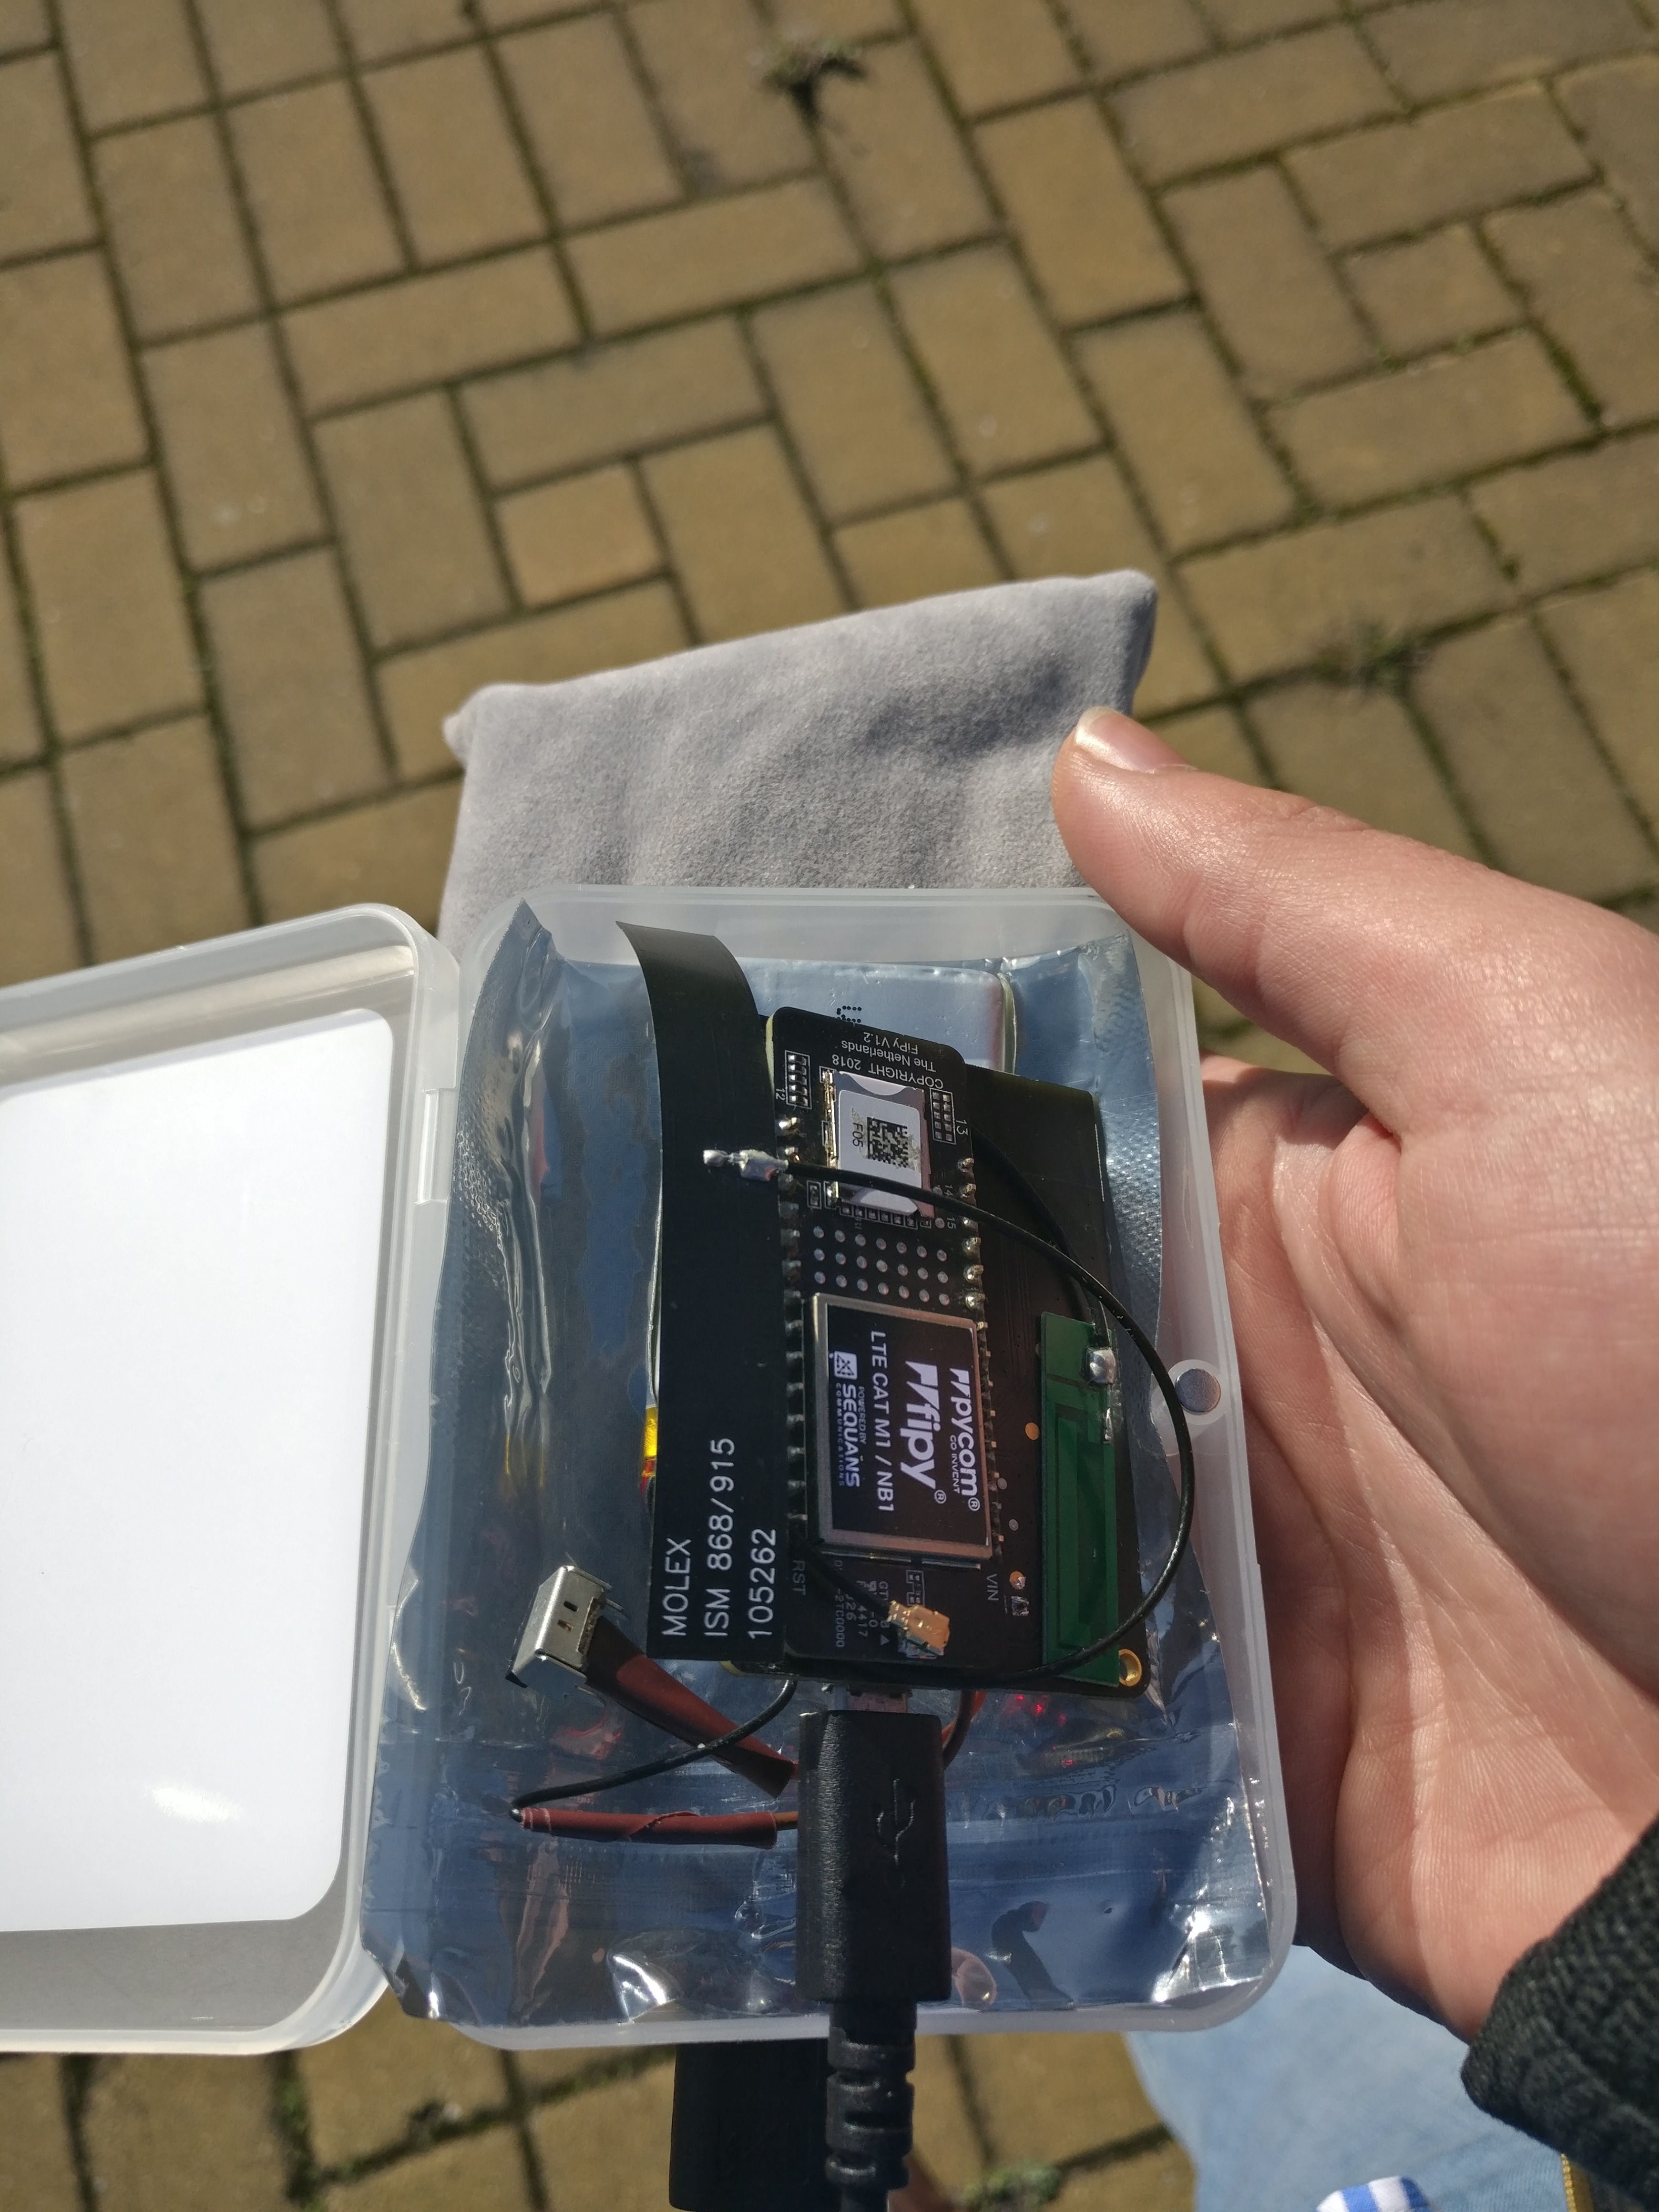
\includegraphics[width=0.5\linewidth]{Chapters/Figures/IMG_20191205_140631.jpg}}%
    }
  \caption{A figure !}
  \label{fig:test5}
\end{figure}


\begin{figure}[htbp]
  \centering
    \scalebox{0.6}{
    {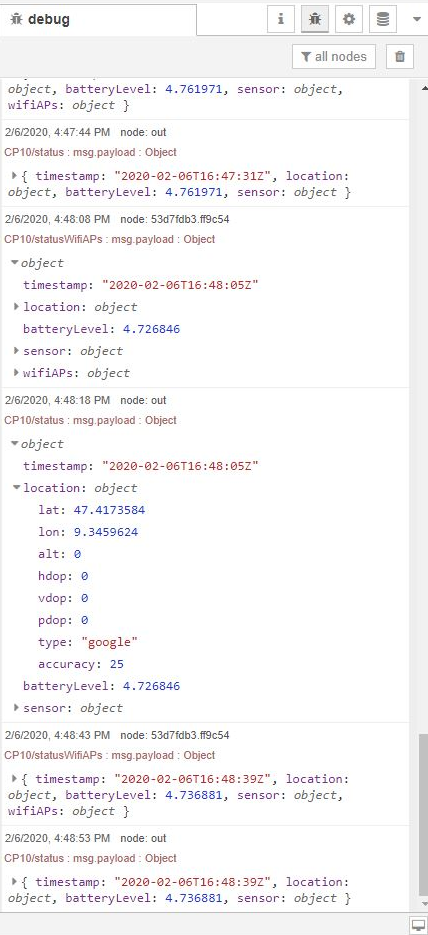
\includegraphics[width=0.5\linewidth]{Chapters/Figures/CP10swiss.png}}%
    }
  \caption{A figure !}
  \label{fig:node_red_debug1}
\end{figure}
\newpage
\begin{figure}[htbp]
  \centering
  
    {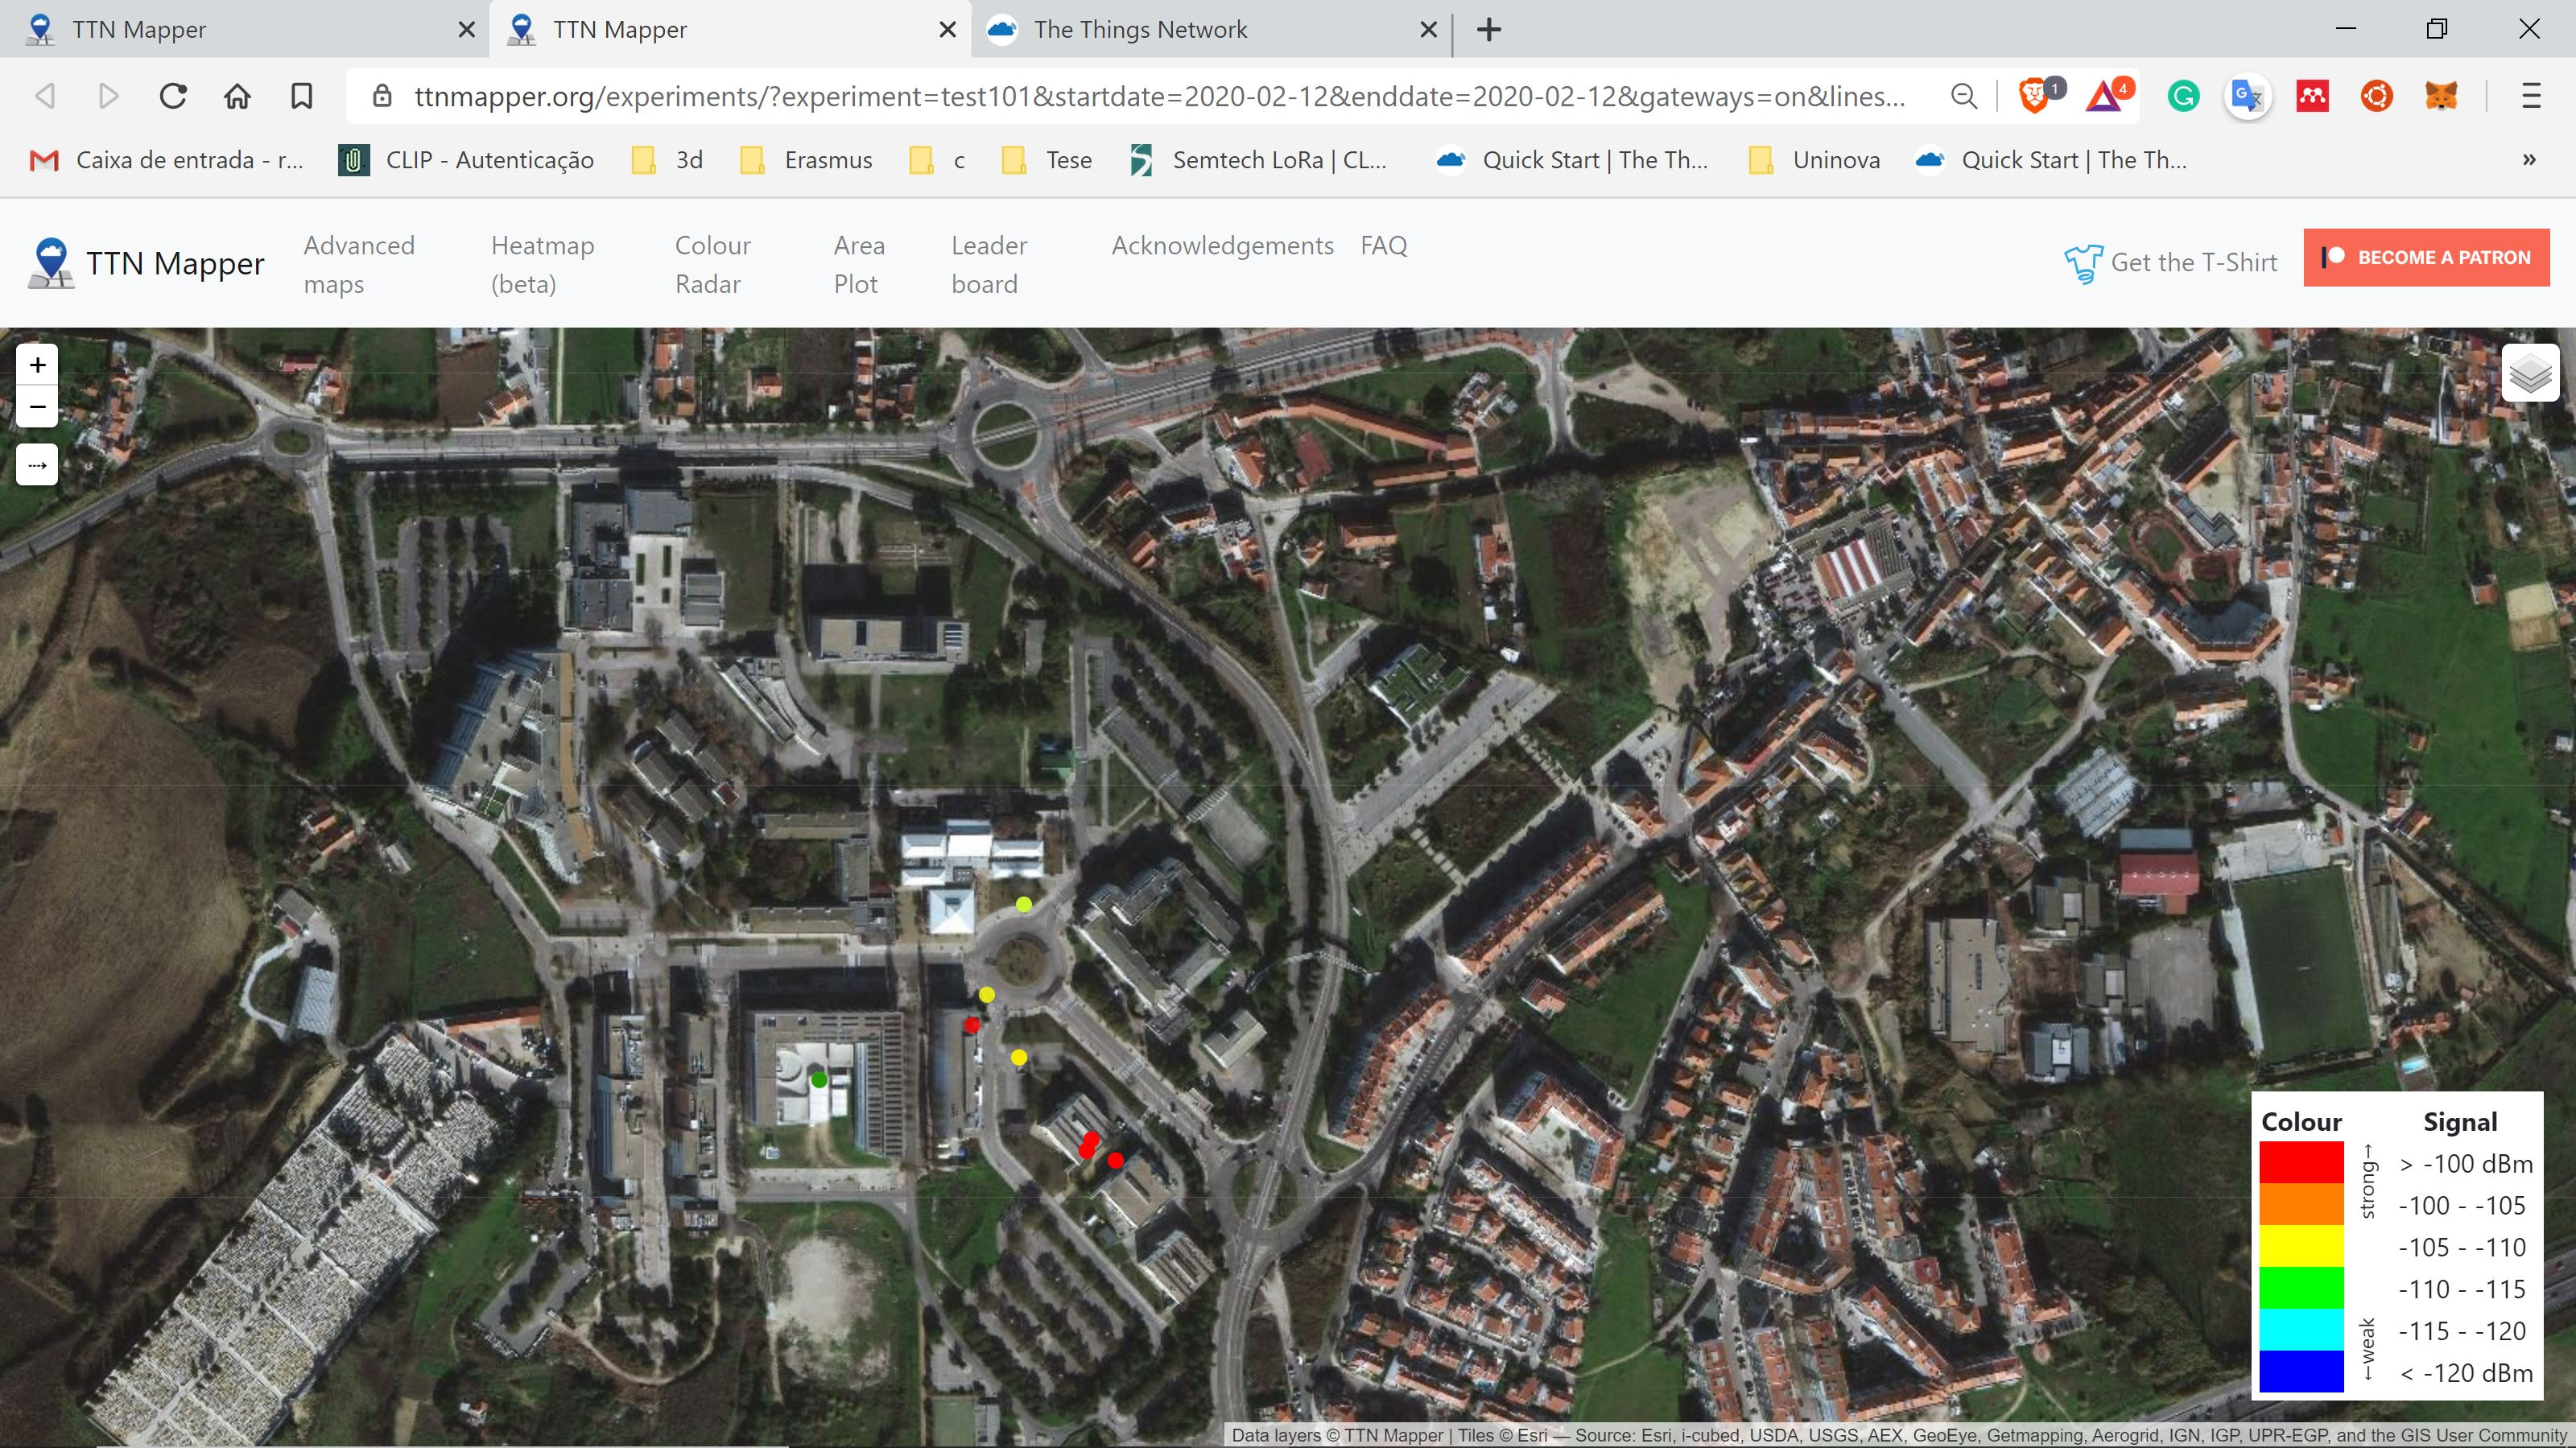
\includegraphics[width=0.5\linewidth]{Chapters/Figures/ttnmapper.JPG}}%
 
  \caption{A figure !}
  \label{fig:ttn_mapper}
\end{figure}



\begin{figure}[htbp]
  \centering
  
    {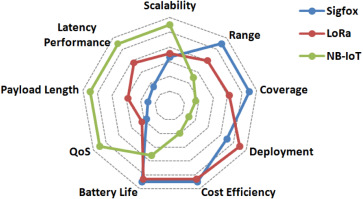
\includegraphics[width=0.5\linewidth]{Chapters/Figures/radar1.jpg}}%
 
  \caption{radar LPWAN}
  \label{fig:radar1}
\end{figure}



\begin{figure}[htbp]
  \centering
  
    {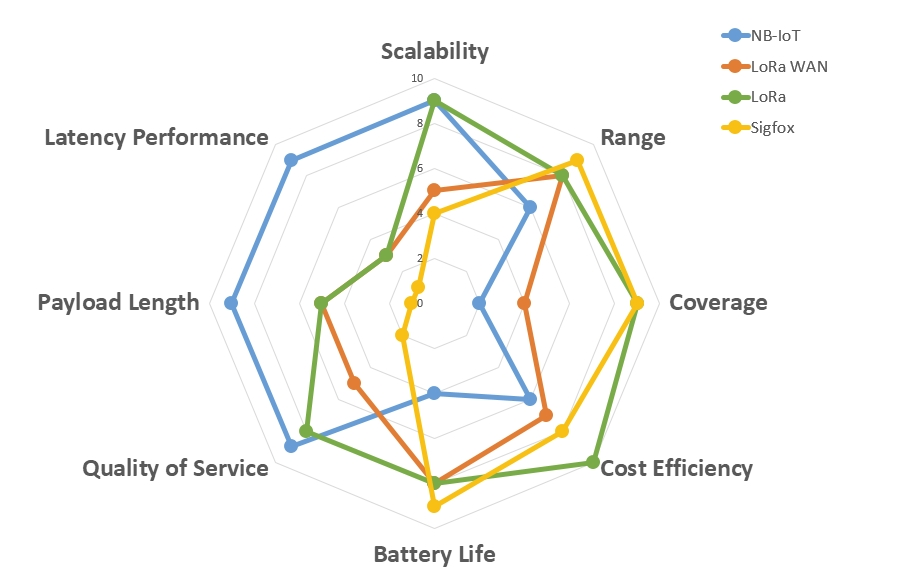
\includegraphics[width=0.5\linewidth]{Chapters/Figures/radar2.jpg}}%
 
  \caption{radar LPWAN 2}
  \label{fig:radar2}
\end{figure}

\begin{figure}[htbp]
  \centering
  
    {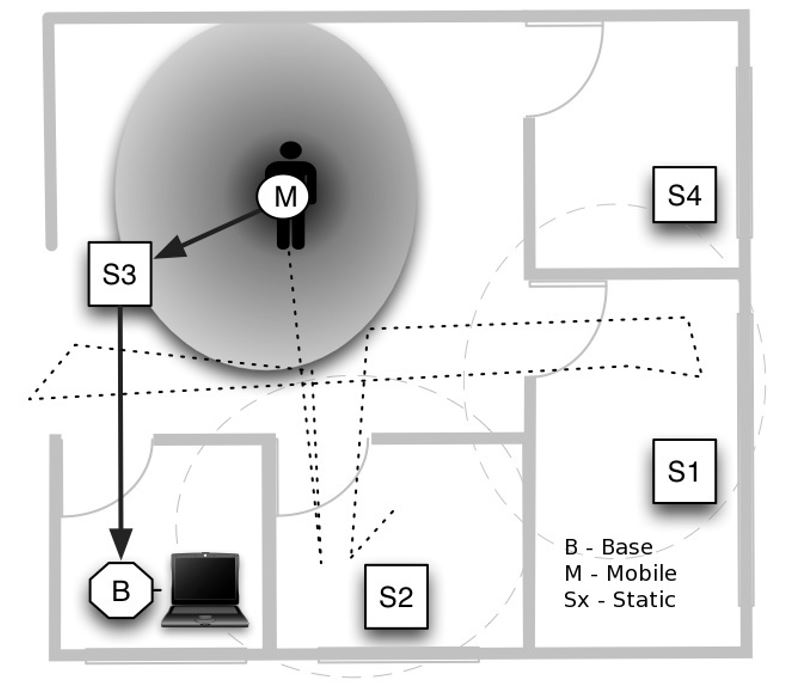
\includegraphics[width=0.5\linewidth]{Chapters/Figures/indoor.JPG}}%
 
  \caption{indoor}
  \label{fig:indoor}
\end{figure}

%%%%%%%%%%%% DT 
\begin{figure}[htbp]
  \centering
  
    {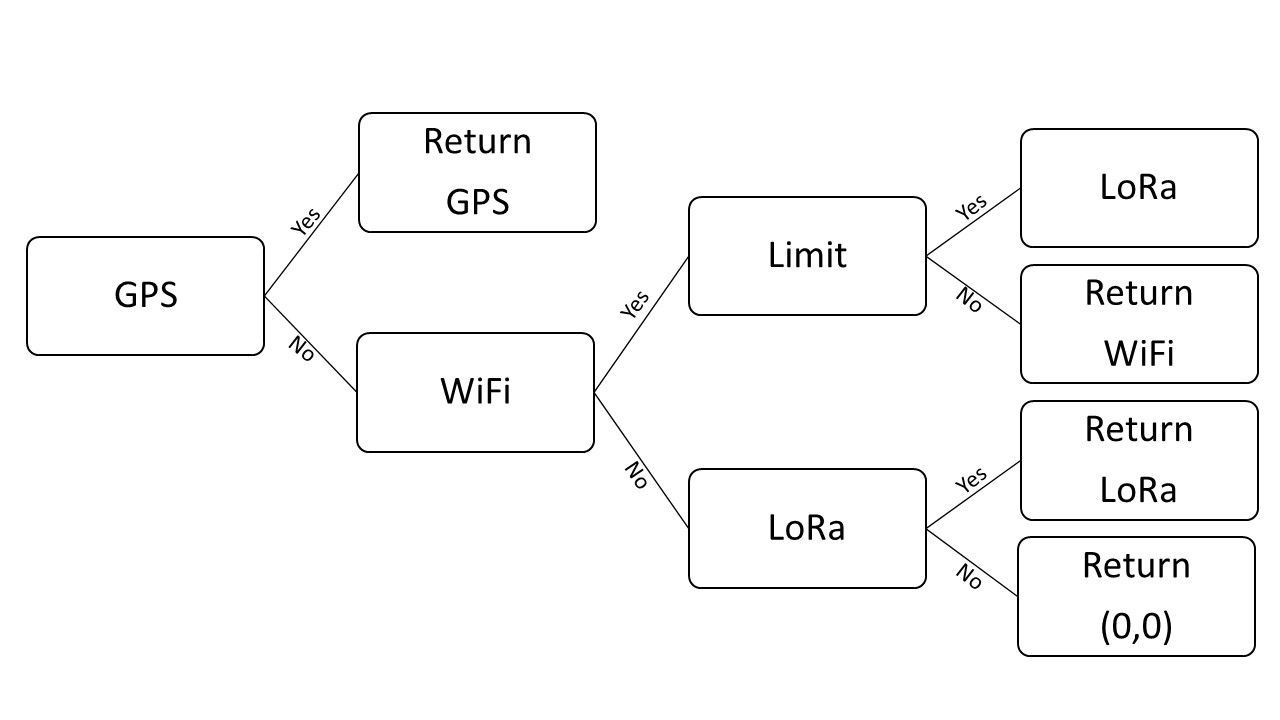
\includegraphics[height= 2.4in,width=0.9\linewidth]{Chapters/Figures/Stage1tree.jpg}}%
 
  \caption{Stage 1 Decission tree}
  \label{fig:Stage1_DT}
\end{figure}

 In the Figure~\ref{fig:Stage1_DT}, is represented the tree behind the Adaptive Geolocation Solver, for this stage. 
 \newline\newline\newline 
%###### telemovel ###


%\begin{figure}[htbp]
% \centering
% \scalebox{0.5}{
%  {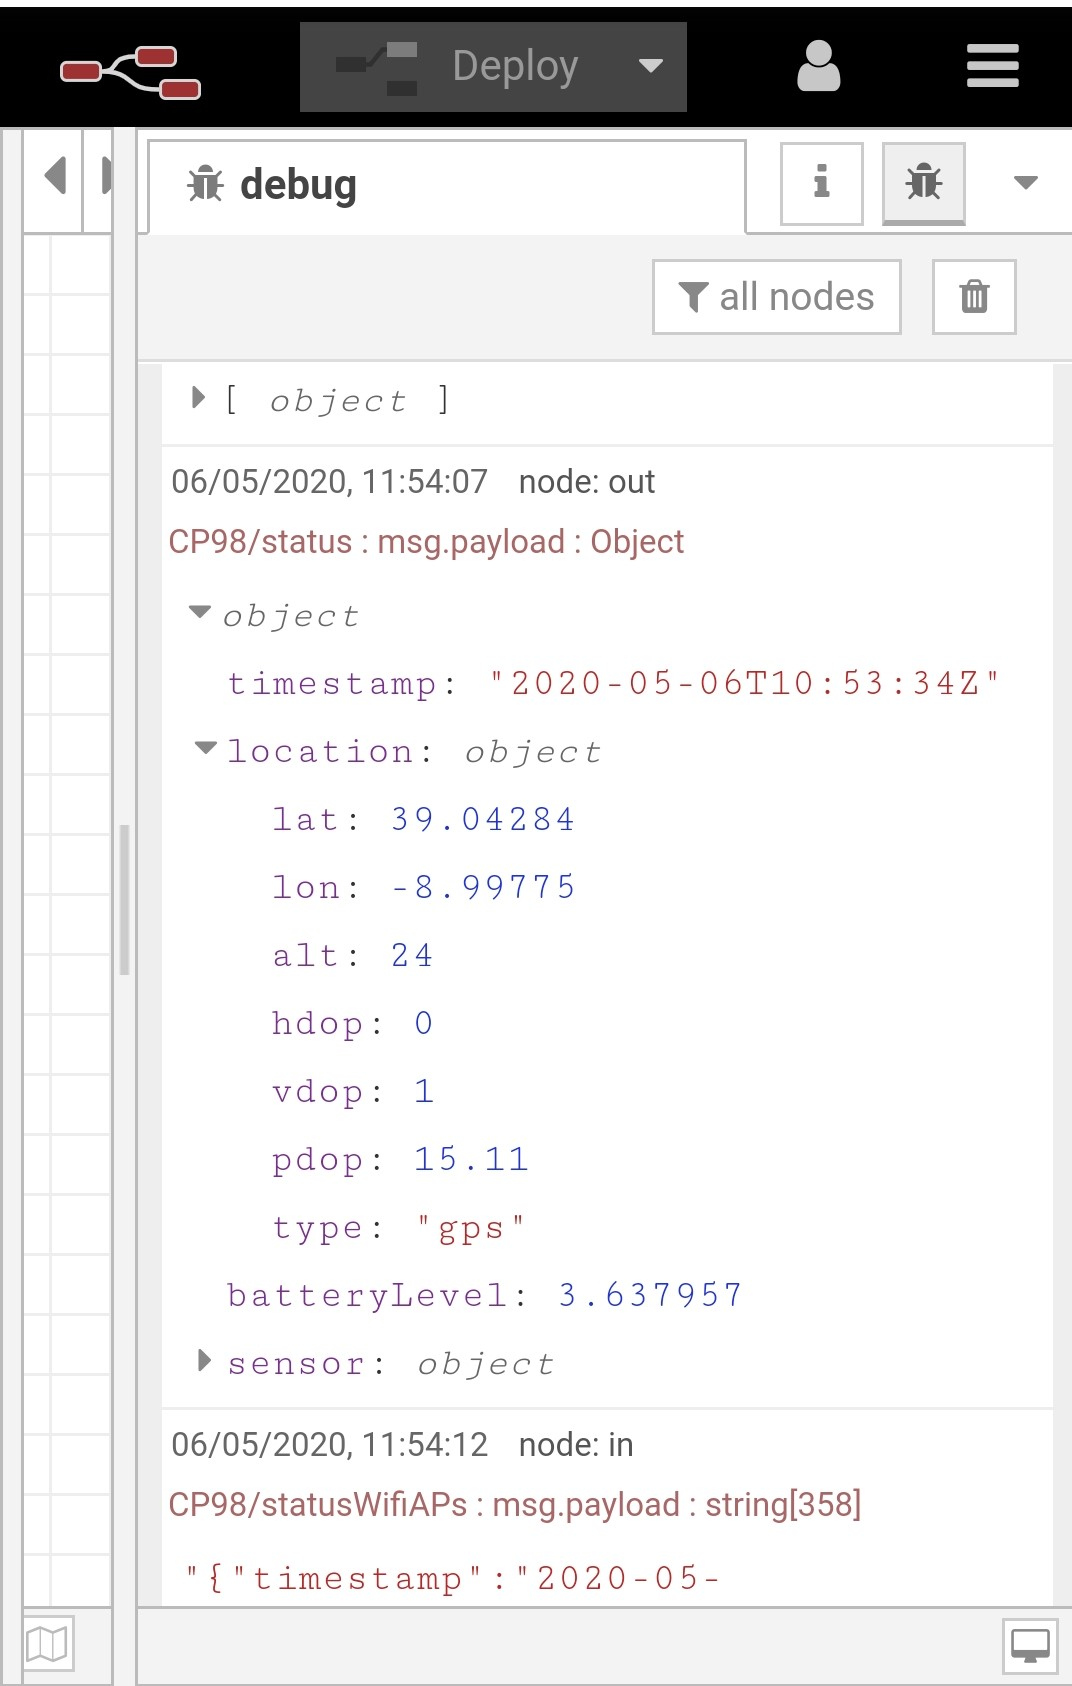
\includegraphics[width=0.5\linewidth]{Chapters/Figures/gpsnodered.jpg}}%
%  }
%  \caption{GPS Node Red}
% \label{fig:gpsnodered}
%\end{figure}
%\begin{figure}[htbp]
%  \centering
%  \scalebox{0.5}{
%    {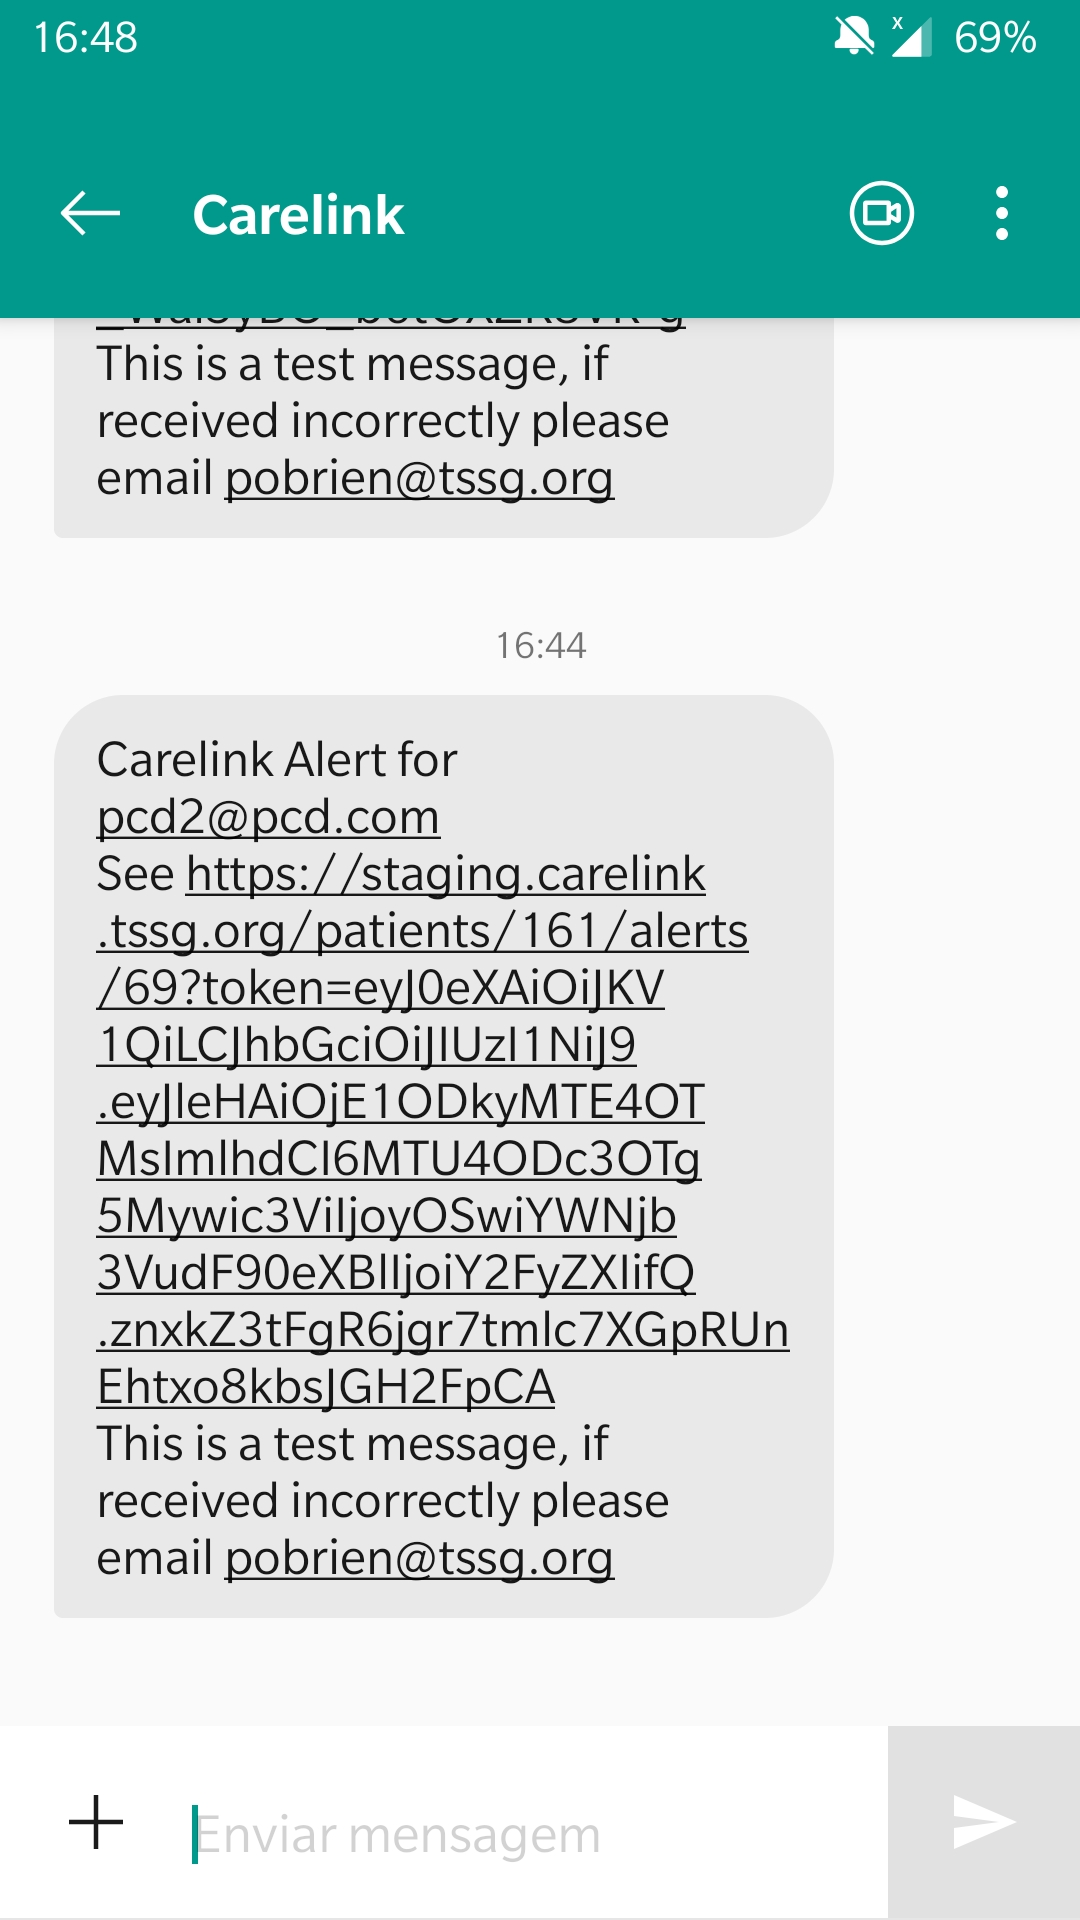
\includegraphics[width=0.5\linewidth]{Chapters/Figures/smsalert.jpg}}%
%    }
%  \caption{SMS Alert}
%  \label{fig:sms}
%\end{figure}
%\begin{figure}[htbp]
 % \centering
%  \scalebox{0.5}{
%    {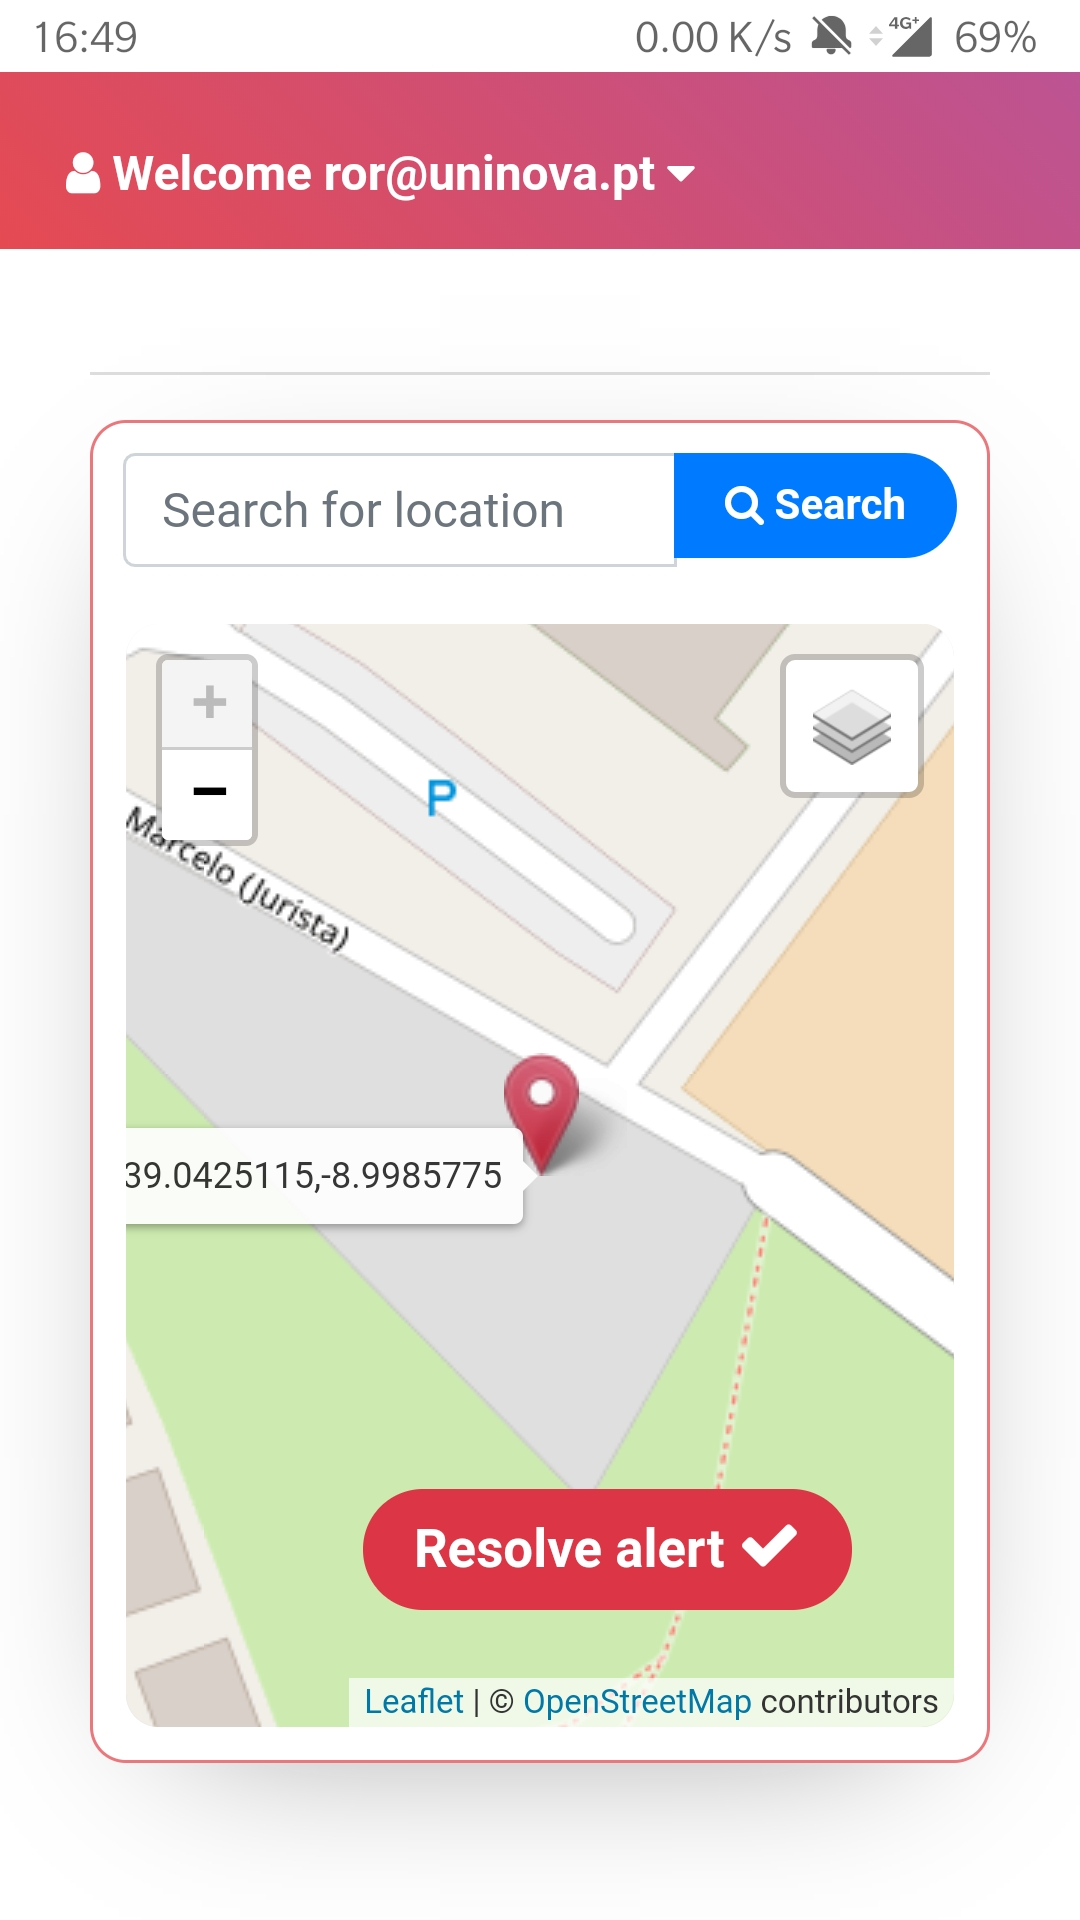
\includegraphics[width=0.5\linewidth]{Chapters/Figures/webalert.jpg}}%
%    }
 % \caption{web Alert}
 % \label{fig:web Alert}
%\end{figure}





